\documentclass{fisatproject}
\usepackage{graphicx}
\title{Peer2Chat - Decentralized Chat App }
\team{Dharwish Raj - FIT17CS046 \\ Adhyaksh Guhan - FIT17CS007 \\ Alan Raphael - FIT15CS015 \\ Ajay Diji - FIT17CS009}
\author{Dharwish Raj(FIT17CS046), Adhyaksh Guhan(FIT17CS007), Alan Raphael(FIT15CS015), Ajay Diji(FIT17CS009)}
\begin{document}
\maketitle

\makecert

\newpage
%\thispagestyle{plain}
\pagenumbering{roman}
\setcounter{page}{1}
\newgeometry{top=4cm,bottom=0.1cm}
\renewcommand\abstractname{ABSTRACT}
\begin{abstract}
\vspace{5cm}
A decentralised application is one that does lies outside the purview and control of a single authority. This enables the app to allow for transfer of data with complete anonimity and interruptions from third-parties. This project uses a peer-to-peer (p2p) network to enable communication between multiple parties in a decentralised fashion.
\end{abstract}


\newpage
%\thispagestyle{plain}
\renewcommand\abstractname{ACKNOWLEDGMENT}
\begin{abstract}
\vspace{5cm}
If words are considered as symbols of approval and tokens of acknowledgment , then let the words play the heralding role of expressing our gratitude. \\ \\
 \textbf{Ms. Anitha P}, Chairman, Governing Body-FISAT, who provided us with vital facilities required by the project right from the inception to completion. \\ \\
 We express our deepest appreciation towards \textbf{Dr. George Issac}, Principal ,FISAT, for providing amenities, which helped us in the fulfillment of our project. \\ \\
 \textbf{Dr. Prasad J.C} , Head of Department of Computer Science and Engineering, FISAT, guided us  and rendered his help in all phases of our project. \\ \\
 We would also like to express our gratitude to \textbf{Ms. Sruthy Suresh , Ms. Divya John}, had been a pillar of support for the successful completion of our project. \\ \\
 Last but not the least, we express our sincere gratitude to all the staffs of the Department of Computer Science  and Engineering, who helped us in the course of work. \\ \\

\vspace{1cm}
\begin{flushright}
Dharwish Raj(FIT17CS046)

Adhyaksh Guhan(FIT17CS007)

Alan Raphael(FIT15CS015)

Ajay Diji(FIT17CS009)
\end{flushright}
\end{abstract}
\newpage

\restoregeometry
\tableofcontents

\newpage
\pagestyle{fancy}


\chapter{INTRODUCTION}
\pagenumbering{arabic}
\setcounter{page}{1}
\renewcommand{\baselinestretch}{1.50}
\section{Overview}
Decentralised networks, as opposed to centralised networks, are organised in a much more distributed fashion. Each node within the network functions as a separate authority with independent decision-making power regarding how it interacts with other systems. These networks also distribute processing power and workload functions among connected servers. This creates a lack of any central power that can maintain control over the whole network and control how information flows within it. The P2P based chat app utlises this philosophy and can connect one peer to another to start a conversation in complete anonimity.

	\subsection{Peer-to-peer}
	Peer-to-peer (P2P) computing or networking is a distributed application architecture that partitions tasks or workloads between peers. Files can be shared directly between systems on the network without the need of a central server. In other words, each computer on a P2P network becomes a file server as well as a client.
	
	\begin{center}
		\begin{figure}[h]
			
			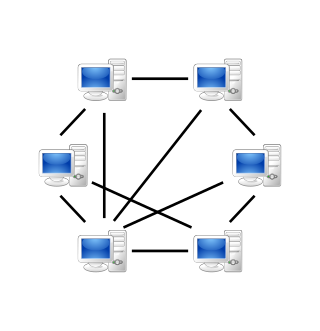
\includegraphics[width=8.2cm]{p2p.png}
			\caption{A p2p network}
			
		\end{figure}
	\end{center}
	The only requirements for a computer to join a peer-to-peer network are an Internet connection and P2P software. Common P2P software programs include Kazaa, Limewire, BearShare, Morpheus, and Acquisition. Once connected to the network, P2P software allows a user to search for files on other people's computers. Meanwhile, other users on the network can search for files on the user's computer, but typically only within a single folder that is designated to share. 
	
	\subsection{Advantages}

	\begin{itemize}
		\item \textbf{Easy of setup and maintanence}
		The network is fast and inexpensive to setup and maintain as it requires no dedicated servers since all users act as both client and server.
		
		\item \textbf{More reliable}
		The failure of a single peer in the network does not affect all other peers in the rest of the network due its decentralised nature.
		
		\item \textbf{Access to shared resources}
		The user can control their shared resources and can set any resource as accessible as long as it is in a shared folder. This negates the need of a System Administrator.
		
	\end{itemize}
	
	\begin{center}
		\begin{figure}[h]
			
			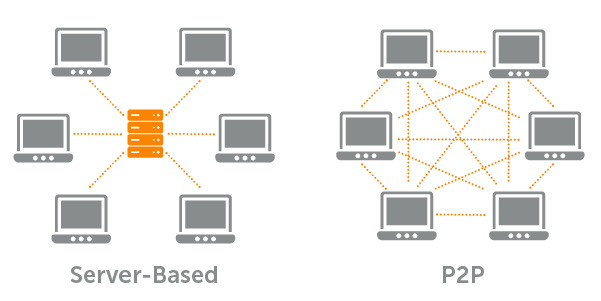
\includegraphics[scale=.75]{svp.jpg}
			\caption{Server based vs P2P}
			
		\end{figure}
	\end{center}


\chapter{RELATED WORK}

\begin{itemize}
	\item \textbf{1. Augur}
	Augur combines decentralized networking and financial prediction markets to create powerful forecasting. It’s built upon the Ethereum blockchain. In its current guise, Augur allows you to make predictions about real-world events not limited to financial markets. The platform turns your prediction into “shares” that other users can buy or sell.
	

	\item \textbf{2. Vett.space}
	This is that game made online. It's an online multiplayer implementation of Dots-and-Boxes !
	Built with VueJS, d3.js, P2PT. Uses WebTorrent trackers for making Peer-to-Peer connections for multiplayer.
	

	\item \textbf{3. Aragon}
	
	Aragon is an ambitious decentralized management platform, also built on the Ethereum blockchain. It wants to break down the traditional barriers that restrict the creation and maintenance of organizational structures. In other words, Aragon wants to make it easier to create private Decentralized Autonomous Organizations (DAOs), along with everything you need to succeed. This means arbitration, token management and transfers, role assignments, fundraising, and much more.

	\item \textbf{4. Sia}
	
	Sia is a promising decentralized storage platform that leverages “underutilized hard drive capacity around the world,” creating a first-of-its-kind blockchain-based data storage marketplace. The platform turns those empty hard drives into cheap cloud storage that almost anyone can use. Prices are cheap, especially when compared to other major cloud storage providers.
	
	\item \textbf{5. SAFE Network}
	
	The SAFE Network uses a decentralized approach to protecting consumer data and private communication. SAFE, which stands for Secure Access For Everyone, uses peer-to-peer technology to share that computing power between connected users. This creates a secure private network, rather than relying on centralized servers.
\end{itemize}


\chapter{DESIGN and IMPLEMENTATION}

\section{Design}

Peer2Chat is implemented using following technologies : 
  \begin{itemize}
 \item A web peer2peer communicating library called p2pt which developed using WebTorrent modules 
 \item A JavaScript program that initiate Torrent trackers and accept peer list and packets passed
 \item A web application interface for above programe runs on Vue.js 
 \end{itemize}

   \subsection{How this works}
   
    	\subsubsection{Peer-to-Peer Communication}
   WebTorrent is a library which created a new kind of Torrent Trackers called \textbf{"WebSocket Trackers"}  also known as "WebTorrent Trackers". Most of the torrent clients are using this technology to share files. But web-based  clients have a limitation that it  JavaScript in browser can't directly make TCP/IP connections and communicate. To overcome this problem, we use WebRTC. WebRTC is the method by which browsers can communicate to other browsers peer to peer (P2P). WebTorrent makes use of WebRTC for sharing Torrents on web. But to establish peer2peer connection between WebRTC a signalling server is needed. To avoid that we use WebSocket trackers as the singling servers to establish communication between clients.  
   		\subsubsection{Finding Clients (Peers)}
   		We use a magnet link. The magnet link has a unique identifier for our torrent called the \textbf{Info Hash}. This ID will be unique for all torrents.
   		
   		Similarly, to implemented chat app, we use an identifier. This identifier is converted to a valid Info Hash and sent to our WebTorrent trackers who will give us a list of web peers. These web peers would be the other users also using our app.



   \vspace{1cm}
  
 
    
    \vspace{1cm}
    \subsection{User Interface}
    The front-end interface of our chat application is build using Vue.js, which will help single page navigation compared to regular HTML/CSS.
    \newpage

\section{Implementation}
    What is basically happening here is that when client load this app, Trackers will pass InfoHash to the new client which contains manget link.
    
        \vspace{0.6cm}
Announcing Trackers URL in app.js  
	\begin{lstlisting}[language=java]
	let announceURLs = [
	"wss://tracker.openwebtorrent.com",
	"wss://tracker.sloppyta.co:443/announce",
	"wss://tracker.novage.com.ua:443/announce",
	"wss://tracker.btorrent.xyz:443/announce",
	]
	if (window.location.hostname === "localhost") {
	announceURLs = ["ws://localhost:5000"]
   });
   \end{lstlisting}
           \vspace{0.6cm}
   Magnet link will help to generate peer list (connected clients) on every client, so that it will establish communication with peers (clients using WebRTC)
   
   
              \vspace{0.6cm}
              Connect to network and start discovering peers in p2pt
	 \begin{lstlisting}[language=java]
	 start () {
	 const $this = this
	 
	 this.on('peer', (peer) => {
	 var newpeer = false
	 if (!$this.peers[peer.id]) {
	 newpeer = true
	 $this.peers[peer.id] = {}
	 $this.responseWaiting[peer.id] = {}
	 }
	 
	 peer.on('connect', () => {
	 $this.peers[peer.id][peer.channelName] = peer
	 
	 if (newpeer) {
	 $this.emit('peerconnect', peer)
	 }
	 })
	    \end{lstlisting}
        \vspace{0.6cm}

    

Next we implementing function to join, send and revive data between client in App.js
         \vspace{0.6cm}
 	 \begin{lstlisting}[language=java]
 	 
 	 \end{lstlisting}


\chapter{TESTING}
The project was implemented by testing at multiple stages.
First a testing was done as soon as a client could be connected to the server, which displayed the client was connected as soon as a server client connection was established.


Then multiple clients were connected to the same server and tested



After this an app with a similar UI to our familiar chat apps were made, with a handle so that the user can identify who is broadcasting the given message.
\chapter{RESULTS}


The final result of the project is a broadcasting app that basically comprises of a server and multiple clients. Multiple clients can connect to a single server, can give their own names and also send and receive messages.The broadcasting app uses Socket.io to connect the server to the clients.Such a system can be used in institutions for Broadcasting important information between the faculty and the students using a LOCAL AREA NETWORK.












\chapter{CONTRIBUTIONS}

Each member of team had contributed equally to the project. The parts that were worked on were the vue.js code, HTML and the p2p script to call the webtrackers for the webRTC. 






\chapter{CONCLUSION}

Decentralised networks can be an effective method of communication and sharing that prioritises encryption and privacy for all users. The growing number of privacy concerns due to the actions of various central powers can negated through the use of these networks, especially since they are fast and inexpensive to setup and maintain. This chatting app can enable easy communication and data sharing while also being inexpensive and safe to use for all involved users.
\newpage



\begin{thebibliography}{1}
	\bibitem{nist} Christensson, Per. "P2P Definition." TechTerms. Sharpened Productions, 2006. Web. 16 June 2020. 
	\url{https://techterms.com/definition/p2p}
	
\end{thebibliography}


\begin{appendices}
\chapter{Sample Code}
\section{index.js}
\begin{lstlisting}[language=c++]

const express = require('express');
const socket = require('socket.io');
let clients = 0;
const app = express();
const server = app.listen(4000,function(){
   console.log("listening to the request on port 4000");
});

//static files

app.use(express.static('public'));

const io = socket(server);


io.on('connection',function(socket){

   socket.on('chat',function(data){
           io.sockets.emit('chat',data);
   });

   socket.on('typing', function(data){
      socket.broadcast.emit('typing', data);
   });
});

\end{lstlisting}
\newpage
\section{chat.js}
\begin{lstlisting}[language=c++]


const socket = io.connect('http://localhost:4000');

//Query DOM
const message = document.getElementById('message');
const handle = document.getElementById('handle');
const sendButton = document.getElementById('send');
const output = document.getElementById('output');
const announcements = document.querySelectorAll('.announcements');
const feedback = document.getElementById('feedback');
const rightPanel = document.getElementById('right-panel');
//create date object
const date = new Date().toDateString();

//emit events

sendButton.addEventListener('click',function(){
    if(message.value.length > 0 & handle.value.length > 0){
        socket.emit('chat', {
            message: message.value,
            handle: handle.value
        });
      }
      message.value = "";
});

message.addEventListener('keypress', function(){
    if(handle.value.length > 0){
      socket.emit('typing', handle.value);
    }
  });

//listen for events

socket.on('chat',function(data){
    feedback.innerHTML = '';
    output.innerHTML +='<li>'+'<div class="chat-body clearfix">'+'<div class="header">'+'<small class=" text-muted">'+'<span class="glyphicon glyphicon-time">'+'</span>'+ date +'</small>'+' <strong class="pull-right primary-font">'+data.handle+'</strong>' +'</div>'+'<p>'+ data.message + '</p>'+'</div>'+'</li>';
});

socket.on('typing', function(data){
    feedback.innerHTML = '<p><em>' + data + ' is typing a message...</em></p>';
});

\end{lstlisting}
\newpage


\section{index.html}
\begin{lstlisting}[language=c++]


<!DOCTYPE html>
<html lang="en">
   <head>
      <meta charset="UTF-8">
      <meta name="description" content="Chat">
      <meta name="keywords" content="HTML,CSS,JavaScript,SOCKET.IO">
      <meta name="viewport" content="width=device-width, initial-scale=1.0">
      <title>Broadcast App</title>
      <script src="/socket.io/socket.io.js"></script>
      <!-- Latest compiled and minified CSS -->
      <link rel="stylesheet" href="https://maxcdn.bootstrapcdn.com/bootstrap/4.0.0/css/bootstrap.min.css" integrity="sha384-Gn5384xqQ1aoWXA+058RXPxPg6fy4IWvTNh0E263XmFcJlSAwiGgFAW/dAiS6JXm" crossorigin="anonymous">
      <link href="https://maxcdn.bootstrapcdn.com/font-awesome/4.4.0/css/font-awesome.min.css" rel="stylesheet">
      <link rel="stylesheet" href="https://use.fontawesome.com/releases/v5.8.1/css/all.css" integrity="sha384-50oBUHEmvpQ+1lW4y57PTFmhCaXp0ML5d60M1M7uH2+nqUivzIebhndOJK28anvf" crossorigin="anonymous">
      <link href="/styles.css" rel="stylesheet" >
   </head>
   <body>
      <div class="container-fluid header-container px-0">
         <div class="row mx-0">
            <div class="col-sm-12 px-0">
               <div class="row">
                  <div class="col-sm-3">
                  </div>
                  <div class="col-sm-6">
                     <br> <br>
                     <h1 class="header-text">Broadcast app</h1>
                  </div>
               </div>
            </div>
            <!-- end of col-sm-12 -->
         </div>
         <!-- end of row -->
      </div>
      <!-- end of container> -->
       <div>
       <p id="feedback"></p>
      </div>
      <div class="container-fluid" id="output-container">
         <div class="row no-gutters">
            <div class="col-sm-3 side" id="left-panel"></div>
            <div class="col-sm-6" id="main-output">
               <div class="row output-row no-gutters">
                  <div class="col-sm-12"id="output">
                     <p class="announcements"></p>
                  </div>
               </div>
               <!-- end of row -->
               <div class="row no-gutters">
                  <div class="col-sm-10" id="changecolour">
                     <textarea id="message" type="text" placeholder="Message"></textarea>
                  </div>
                  <!-- end of col-sm-6-->
                  <div class="col-sm-2 no-gutters" id="action-here">
                     <input id="handle" type="text" placeholder="Handle" />
                     <button class="btn-btn-success btn-block" id="send">Send</button>
                  </div>
                  <!--end of col-sm-12 -->
               </div>
               <!-- end of nested row -->
            </div>
            <!-- end of col-sm-8 -->
            <div class="col-sm-3 side" id="right-panel"></div>
         </div>
         <!-- end of row -->
      </div>
      <!-- end of container -->
      <script src="/chat.js"></script>
      <!-- jQuery library -->
      <script src="https://ajax.googleapis.com/ajax/libs/jquery/3.3.1/jquery.min.js"></script>
      <!-- Latest compiled JavaScript -->
      <script src="https://maxcdn.bootstrapcdn.com/bootstrap/3.4.0/js/bootstrap.min.js"></script>
   </body>
</html>
\end{lstlisting}
\newpage

\section{style.css}
\begin{lstlisting}[language=c++]

@import url("https://fonts.googleapis.com/css?family=Montserrat:400,400i,700");
body{
  font-family: Montserrat, sans-serif;
  color: rgb(255, 255, 255);
  background-color: rgb(253, 253, 253);
  overflow-x: hidden;
}

.header-container{
  background-image: url("images/kidda.png");
  height:150px;
  border-top: 3px solid rgb(255, 255, 255);

}
.header-text{
  text-transform: uppercase;
  font-weight: 900;
  opacity: 0.7;
  color: #000000;
}

#main-output{
  background-color: rgb(0, 0, 0);
  height: 100%;
}
#output{
  height: 450px;
  overflow-y: scroll;
  width: 50%;
  background-color:#bbbbbb;
  border-bottom: 3px solid rgb(78, 78, 78);
}

.chat
{
    list-style: none;
    margin: 0;
    padding: 0;
}


.chat li .chat-body p
{
    margin: 0;
    color: #777777;
}

.panel .slidedown .glyphicon, .chat .glyphicon
{
    margin-right: 5px;
}
.chat li
{
    margin-bottom: 10px;
    padding-bottom: 5px;
    border-bottom: 1px dotted rgb(169, 178, 179);
}

#message {
    width: 100%;
    height: 100%;
    background-color:#ffffff;
    color: #000000;
}

#send{
  background-color: #3b5998 ;
  color: #FFFFFF;
  margin-left: auto;
  margin-right: auto;
  width: 100%;
  height: 70%;
  margin-top: 0px;
  border: none;
  opacity: 0.7;
}

#changecolour
{
  background-color: #929292;
  height: 75px;
}

#handle{
  width: 100%;
  background-color:rgb(255, 255, 255);
  opacity: 0.9;
  margin-top: 0px;
  margin-left: auto;
  margin-right: auto;
  margin-bottom: 0px;
  height: 30%;
  color:#000000;
}
#date{
font-style: oblique;
color:rgb(0, 0, 0);
font-size: 14px;
}

#style-handle{
  color: rgb(0, 0, 0);
}
.announcements{
    color: #000000;
    text-transform: full-width;
}
#right-panel{
  padding-top: 3px;
  padding: 30px;
  text-align:center;
  color: #ffffff;
  border-top: 2px solid #7289DA;
}
#left-panel{
  padding-top: 3px;
  text-align:center;
  color: #7289DA;
  border-top:2px solid #7289DA;
}
#action-here
{
  background-color: #929292;
}

\end{lstlisting}

\end{appendices}


\end{document}
